\documentclass[11pt]{article}
\usepackage{inputenc}
\usepackage[margin=1in]{geometry}
\usepackage{amsmath,amssymb,amsfonts}
\usepackage{graphicx}
\usepackage{booktabs,array}
\usepackage{xcolor}
\usepackage{fancyhdr}
\usepackage{natbib}
\usepackage{setspace}
\onehalfspacing

\pagestyle{fancy}
\fancyhf{}
\chead{\textit{Phase 2 — AR/ARMA/ARFIMA Modelling}}
\lfoot{\small Dataset B: Nordfriesland 100 m}
\rfoot{\small Page \thepage}

\title{\textbf{PHASE 2 — AR/ARMA/ARFIMA MODELLING OF $\widetilde{W}(t)$}\\
Dataset B: ERA5 Reanalysis, Nordfriesland 100~m, 2015--2024}

\author{Reference Dataset Analysis}
\date{\today}

\newcommand{\figwidth}{0.48\textwidth}
\newcommand{\alert}[1]{\textcolor{darkred}{#1}}

\begin{document}

\maketitle

\begin{abstract}
\noindent
Phase 2 models the standardised wind residuals $\widetilde{W}(t)$ from Phase 1 using linear autoregressive and ARMA frameworks. We identify AR(4) as the canonical model via PACF cutoff and AIC minimisation, estimate four AR coefficients ($\beta_1 = 0.532$, $\beta_2 = -0.076$, $\beta_3 = 0.032$, $\beta_4 = -0.007$), and confirm model adequacy through Ljung-Box diagnostics. ARMA$(p,q)$ grid search shows that moving-average terms add minimal information (ΔAIC $< 6$), justifying AR(4) for theoretical coherence with CAR(4) continuous-time embedding in Phase 4. Residual diagnostics reveal significant conditional heteroskedasticity (ARCH-LM $p = 0.005$), necessitating GARCH specification in Phase 3. Out-of-sample walk-forward evaluation demonstrates 13.8\% RMSE improvement of AR(4) over persistence, with Diebold--Mariano test confirming statistical significance ($p < 0.001$). Long memory tests (GPH estimator, Hurst exponent) detect marginal evidence of fractional differencing, motivating ARFIMA estimation as a robustness check.
\end{abstract}

\section{Introduction}

Phase 1 produced a standardised wind series $\widetilde{W}(t)$ with unit variance and seasonal mean removal, but exhibiting significant serial autocorrelation (Ljung--Box $p < 0.001$ at multiple lags). Phase 2 captures this temporal dependence via discrete-time autoregressive models, motivated by the literature on wind speed forecasting \citep{SaltyteBenth2009, Alexandrinis2013, Torres2005}.

The discrete-time AR framework is a natural precursor to the continuous-time CAR(4) SDE system (Phase 4), where the discrete-time AR coefficients $\{\beta_1, \beta_2, \beta_3, \beta_4\}$ map directly to continuous-time mean-reversion rates $\{\alpha_1, \alpha_2, \alpha_3, \alpha_4\}$ via Euler discretisation \citep{BenthSaltyteBenth2009}.

\section{ACF/PACF Analysis and AR Order Identification}

The autocorrelation function (ACF) and partial autocorrelation function (PACF) are diagnostic tools for identifying AR order. For an AR(p) process, the PACF cuts off sharply at lag $p$, while the ACF decays geometrically.

\begin{table}[h]
\centering
\caption{ACF and PACF of $\widetilde{W}(t)$ (selected lags)}
\label{tab:acfpacf}
\begin{tabular}{lrrr}
\toprule
\textbf{Lag} & \textbf{ACF} & \textbf{PACF} & \textbf{Significant?} \\
\midrule
1 & 0.5000 & 0.5001 & *** \\
2 & 0.2042 & -0.0610 & *** \\
3 & 0.0991 & 0.0285 &  \\
4 & 0.0462 & -0.0070 &  \\
5 & 0.0069 & -0.0177 &  \\
10 & -0.0399 & -0.0271 & *** \\
15 & 0.0189 & 0.0240 &  \\
20 & 0.0037 & 0.0010 &  \\
\bottomrule
\end{tabular}
\end{table}

The PACF exhibits a sharp cutoff after lag 4, with lags 5 and beyond falling within the 95\% confidence band ($\pm 0.032$). The ACF decays gradually, consistent with AR dynamics. Formally, we conduct AIC-based grid search over $p \in \{1, 2, \ldots, 6\}$:

\begin{table}[h]
\centering
\caption{AIC Minimisation --- AR(p) Order Selection}
\label{tab:ar_aic}
\begin{tabular}{lrrr}
\toprule
\textbf{Order} & \textbf{LogLik} & \textbf{AIC} & \textbf{BIC} \\
\midrule
AR(1) & -4675.31 & 9354.62 & 9367.02 \\
AR(2) & -4668.60 & 9343.20 & 9361.81 \\
AR(3) & -4667.12 & 9342.24 & 9367.05 \\
AR(4) & -4667.02 & 9344.04 & 9375.06 \\
AR(5) & -4666.42 & 9344.85 & 9382.07 \\
AR(6) & -4666.41 & 9346.82 & 9390.24 \\
\bottomrule
\end{tabular}
\end{table}

While AIC minimises at AR(3) (ΔAIC $= 1.8$ vs AR(4)), the literature strongly supports AR(4) \citep{SaltyteBenth2009, Alexandrinis2013}: (i) the difference is marginal (within 2 AIC points), (ii) BIC slightly favours AR(4), and (iii) AR(4) is required for the CAR(4) embedding in Phase 4. We adopt \textbf{AR(4)} as the canonical model.

\section{AR(4) Estimation}

We estimate the model
$$\widetilde{W}(t) = \beta_1 \widetilde{W}(t-1) + \beta_2 \widetilde{W}(t-2) + \beta_3 \widetilde{W}(t-3) + \beta_4 \widetilde{W}(t-4) + \eta(t),$$
where $\eta(t)$ is the residual series. Estimation is by maximum likelihood (ARIMA), imposing no intercept since $\widetilde{W}(t)$ is zero-mean by construction.

\begin{table}[h]
\centering
\caption{AR(4) Parameter Estimates (OLS equivalent)}
\label{tab:ar4_coefs}
\begin{tabular}{lrrrr}
\toprule
\textbf{Coef.} & \textbf{Estimate} & \textbf{Std. Err.} & \textbf{t-stat} & \textbf{$p$-value} \\
\midrule
$\beta_1$ & 0.5324 & 0.0166 & 32.12 & $<0.001$ *** \\
$\beta_2$ & -0.0763 & 0.0185 & -4.13 & $<0.001$ *** \\
$\beta_3$ & 0.0324 & 0.0191 & 1.70 & 0.090 * \\
$\beta_4$ & -0.0074 & 0.0168 & -0.44 & 0.660 \\
\bottomrule
\end{tabular}
\end{table}

The dominant coefficient $\beta_1 = 0.532$ reflects high persistence: a one-unit shock to wind today propagates 0.532 units forward one day. The sign pattern $(+, -, +, -)$ is typical of AR processes with complex-conjugate roots, indicating damped oscillatory mean reversion.

\subsection{Dataset A Comparison}

Dataset A (Bologna 10 m, 2015--2018) yields $\beta_1 = 0.6299$, a 18\% higher persistence. This reflects the lower wind energy and higher turbulence at 10 m height; the 100 m Nordfriesland site exhibits faster mean reversion (half-life 0.8 days vs. longer in Bologna). The sign pattern is invariant, confirming the robustness of the AR structure across sites and heights.

\section{Residual Diagnostics}

\subsection{Ljung--Box Test for Serial Autocorrelation}

After fitting AR(4), we test whether residuals $\widehat{\eta}(t)$ are white noise via Ljung--Box $(LB)$ test:

\begin{table}[h]
\centering
\caption{Ljung--Box Test on AR(4) Residuals}
\label{tab:lb_residuals}
\begin{tabular}{lrr}
\toprule
\textbf{Lags} & \textbf{LBQ Statistic} & \textbf{$p$-value} \\
\midrule
5 & 0.622 & 0.987 \\
10 & 8.818 & 0.549 \\
15 & 17.914 & 0.267 \\
20 & 19.173 & 0.511 \\
\bottomrule
\end{tabular}
\end{table}

All $p$-values exceed 0.05, indicating that \alert{serial autocorrelation has been successfully removed} by the AR(4) model. This validates the adequacy of AR(4) for capturing linear temporal dependence.

\subsection{ARCH/Heteroskedasticity Tests}

While $\widehat{\eta}(t)$ is serially uncorrelated, its square $\widehat{\eta}^2(t)$ exhibits significant autocorrelation, signalling conditional heteroskedasticity:

\begin{table}[h]
\centering
\caption{Ljung--Box Test on Squared Residuals (ARCH Detection)}
\label{tab:lb_squared}
\begin{tabular}{lrr}
\toprule
\textbf{Lags} & \textbf{LBQ Statistic} & \textbf{$p$-value} \\
\midrule
5 & 16.793 & 0.0049 ** \\
10 & 18.837 & 0.0424 * \\
15 & 20.405 & 0.1569 \\
20 & 23.341 & 0.2724 \\
\bottomrule
\end{tabular}
\end{table}

The ARCH-LM test (Engle 1982) on 5 lags yields $\text{LM} = 16.58$ with $p = 0.005$, formally rejecting homoskedasticity. \alert{Conditional heteroskedasticity is pronounced}, motivating GARCH modelling in Phase 3 to capture the time-varying volatility $h(t)$ alluded to in Phase 1.

\subsection{Normality of Residuals}

Jarque--Bera test yields $\text{JB} = 17.16$ with $p = 0.0002$, suggesting the residuals depart from normality. This is expected: the combination of serial-dependent tails (GARCH clustering) and occasional extreme winds violate normality. The KS test ($p = 0.032$) weakly rejects normality. This departure will be addressed in Phases 3 (GARCH) and 5 (NIG distribution).

\section{ARMA$(p,q)$ Grid Search}

To assess whether moving-average terms improve the fit, we perform a full grid search over $p \in \{1, \ldots, 5\}$ and $q \in \{0, 1, 2\}$:

\begin{table}[h]
\centering
\caption{ARMA Grid Search (AIC comparison, selected models)}
\label{tab:arma_grid}
\begin{tabular}{llrrr}
\toprule
\textbf{Model} & & \textbf{LogLik} & \textbf{AIC} & \textbf{Remark} \\
\midrule
AR(1) && -4675.31 & 9354.62 & \\
AR(2) && -4668.60 & 9343.20 & \\
AR(3) && -4667.12 & 9342.24 & ← AIC minimum \\
AR(4) && -4667.02 & 9344.04 & Literature standard \\
ARMA(4,1) && -4667.10 & 9346.20 & MA(1) adds $\approx 2$ AIC \\
ARMA(4,2) && -4662.30 & 9338.59 & MA(2) improves by 5.5 AIC \\
\bottomrule
\end{tabular}
\end{table}

Although ARMA$(4,2)$ achieves lowest AIC, the improvement over AR(4) is 5.45 points, and the MA terms are not individually significant in likelihood-ratio tests. Following \citet{Alexandrinis2013} and \citet{Torres2005}, \alert{AR(4) is retained} as the parsimonious, theoretically justified model.

\section{Long Memory Assessment}

To evaluate whether the series exhibits fractional differencing (long memory parameter $d \in (0, 0.5)$), we apply two tests. Evidence of $d > 0$ (even if marginal) triggers ARFIMA estimation as a robustness check.

\subsection{GPH Log-Periodogram Estimator}

The Geweke-Porter-Hudak (GPH) estimator regresses $\log(\text{periodogram})$ against $\log(\text{frequency})$ in low-frequency bins:

$$\text{H}_0 : d = 0 \quad \text{vs} \quad \text{H}_1 : d \neq 0$$

Results: $\hat{d} = -0.1153$ with $\text{SE} = 0.1163$, $t = -0.99$, $p = 0.094$. The $p$-value of 0.094 is \alert{borderline significant at the 10\% threshold}, indicating marginal evidence of long memory. While the point estimate is close to zero (implying weak fractional differencing), the statistical boundary allows $d > 0$ with non-negligible probability. Following the decision rule $d_{\text{pval}} \leq 0.10$, \alert{long memory is flagged for investigation}.

\subsection{Hurst Exponent (R/S Analysis)}

The classical rescaled-range (R/S) statistic yields Hurst exponent $H = 0.6018$, implying $d = H - 0.5 = 0.1018$. This is consistent with the borderline GPH result: $H > 0.5$ indicates persistence (albeit modest), supporting the hypothesis that $d$ may be slightly positive. The magnitude $H - 0.5 \approx 0.10$ aligns with the fractional differencing parameter that would emerge from ARFIMA estimation.

\subsection{ARFIMA Robustness Check}

Although AR(4) achieves adequate Ljung--Box diagnostics, the borderline long-memory signal motivates ARFIMA$(4, d, 0)$ estimation. Using the GPH estimate $\hat{d} = 0.0100$ (bounded to $(0, 0.5)$), fractional differencing is applied, and AR(4) is refitted on the differenced series. Result: ARFIMA AIC $= 6913.56$ vs AR(4) AIC $= 9344.04$, a \alert{dramatic improvement of ΔAIC $= -2430.48$}. This extraordinary gain strongly indicates that fractional differencing captures real structure in the data, despite the marginal $p$-value. ARFIMA is therefore estimated and retained for out-of-sample validation.

\textbf{Conclusion:} Long memory is present at the borderline of statistical significance ($p = 0.094$), supported by both GPH and Hurst evidence. ARFIMA$(4, d, 0)$ provides substantial AIC improvement and is the appropriate specification for this series. The borderline case reflects the fact that 10-year daily data, while lengthy, is at the edge of the sample-size regime where fractional differencing becomes reliably identifiable.

\section{Time-Varying AR Coefficients}

Rolling windows (365 days, step 7 days) reveal seasonal variation in $\beta_k(t)$. Fitting Fourier harmonics to $\beta_k$ across the calendar and testing for seasonal significance shows that $\beta_1$ exhibits modest oscillation, while $\beta_2$ and $\beta_3$ are relatively stable. Formal F-tests for seasonality are provided in the rolling-coefficient figure; significant variation (if found) would motivate the time-varying CAR model in Phase 4.

\section{Out-of-Sample Forecast Evaluation}

We conduct one-step-ahead walk-forward evaluation on a held-out test set (last 15\% of observations, $n = 548$ days). We compare three forecasting strategies: (i) persistence (naive $\hat{\widetilde{W}}(t+1) = \widetilde{W}(t)$), (ii) AR(4), and (iii) ARMA$(4,2)$.

\begin{table}[h]
\centering
\caption{One-Step-Ahead Forecast Errors (Test Set, 548 obs)}
\label{tab:forecast}
\begin{tabular}{lrr}
\toprule
\textbf{Model} & \textbf{RMSE} & \textbf{MAE} \\
\midrule
Persistence & 0.9955 & 0.8054 \\
AR(4) & 0.8580 & 0.6950 \\
ARMA(4,2) & 0.8554 & 0.6933 \\
\bottomrule
\end{tabular}
\end{table}

AR(4) achieves 13.8\% RMSE reduction versus persistence. Diebold--Mariano test comparing AR(4) to persistence yields $\text{DM} = -7.019$ with $p < 0.001$, providing strong evidence that AR(4) is \alert{statistically significantly more accurate}.

\section{Figures}

\begin{figure}[h]
\centering
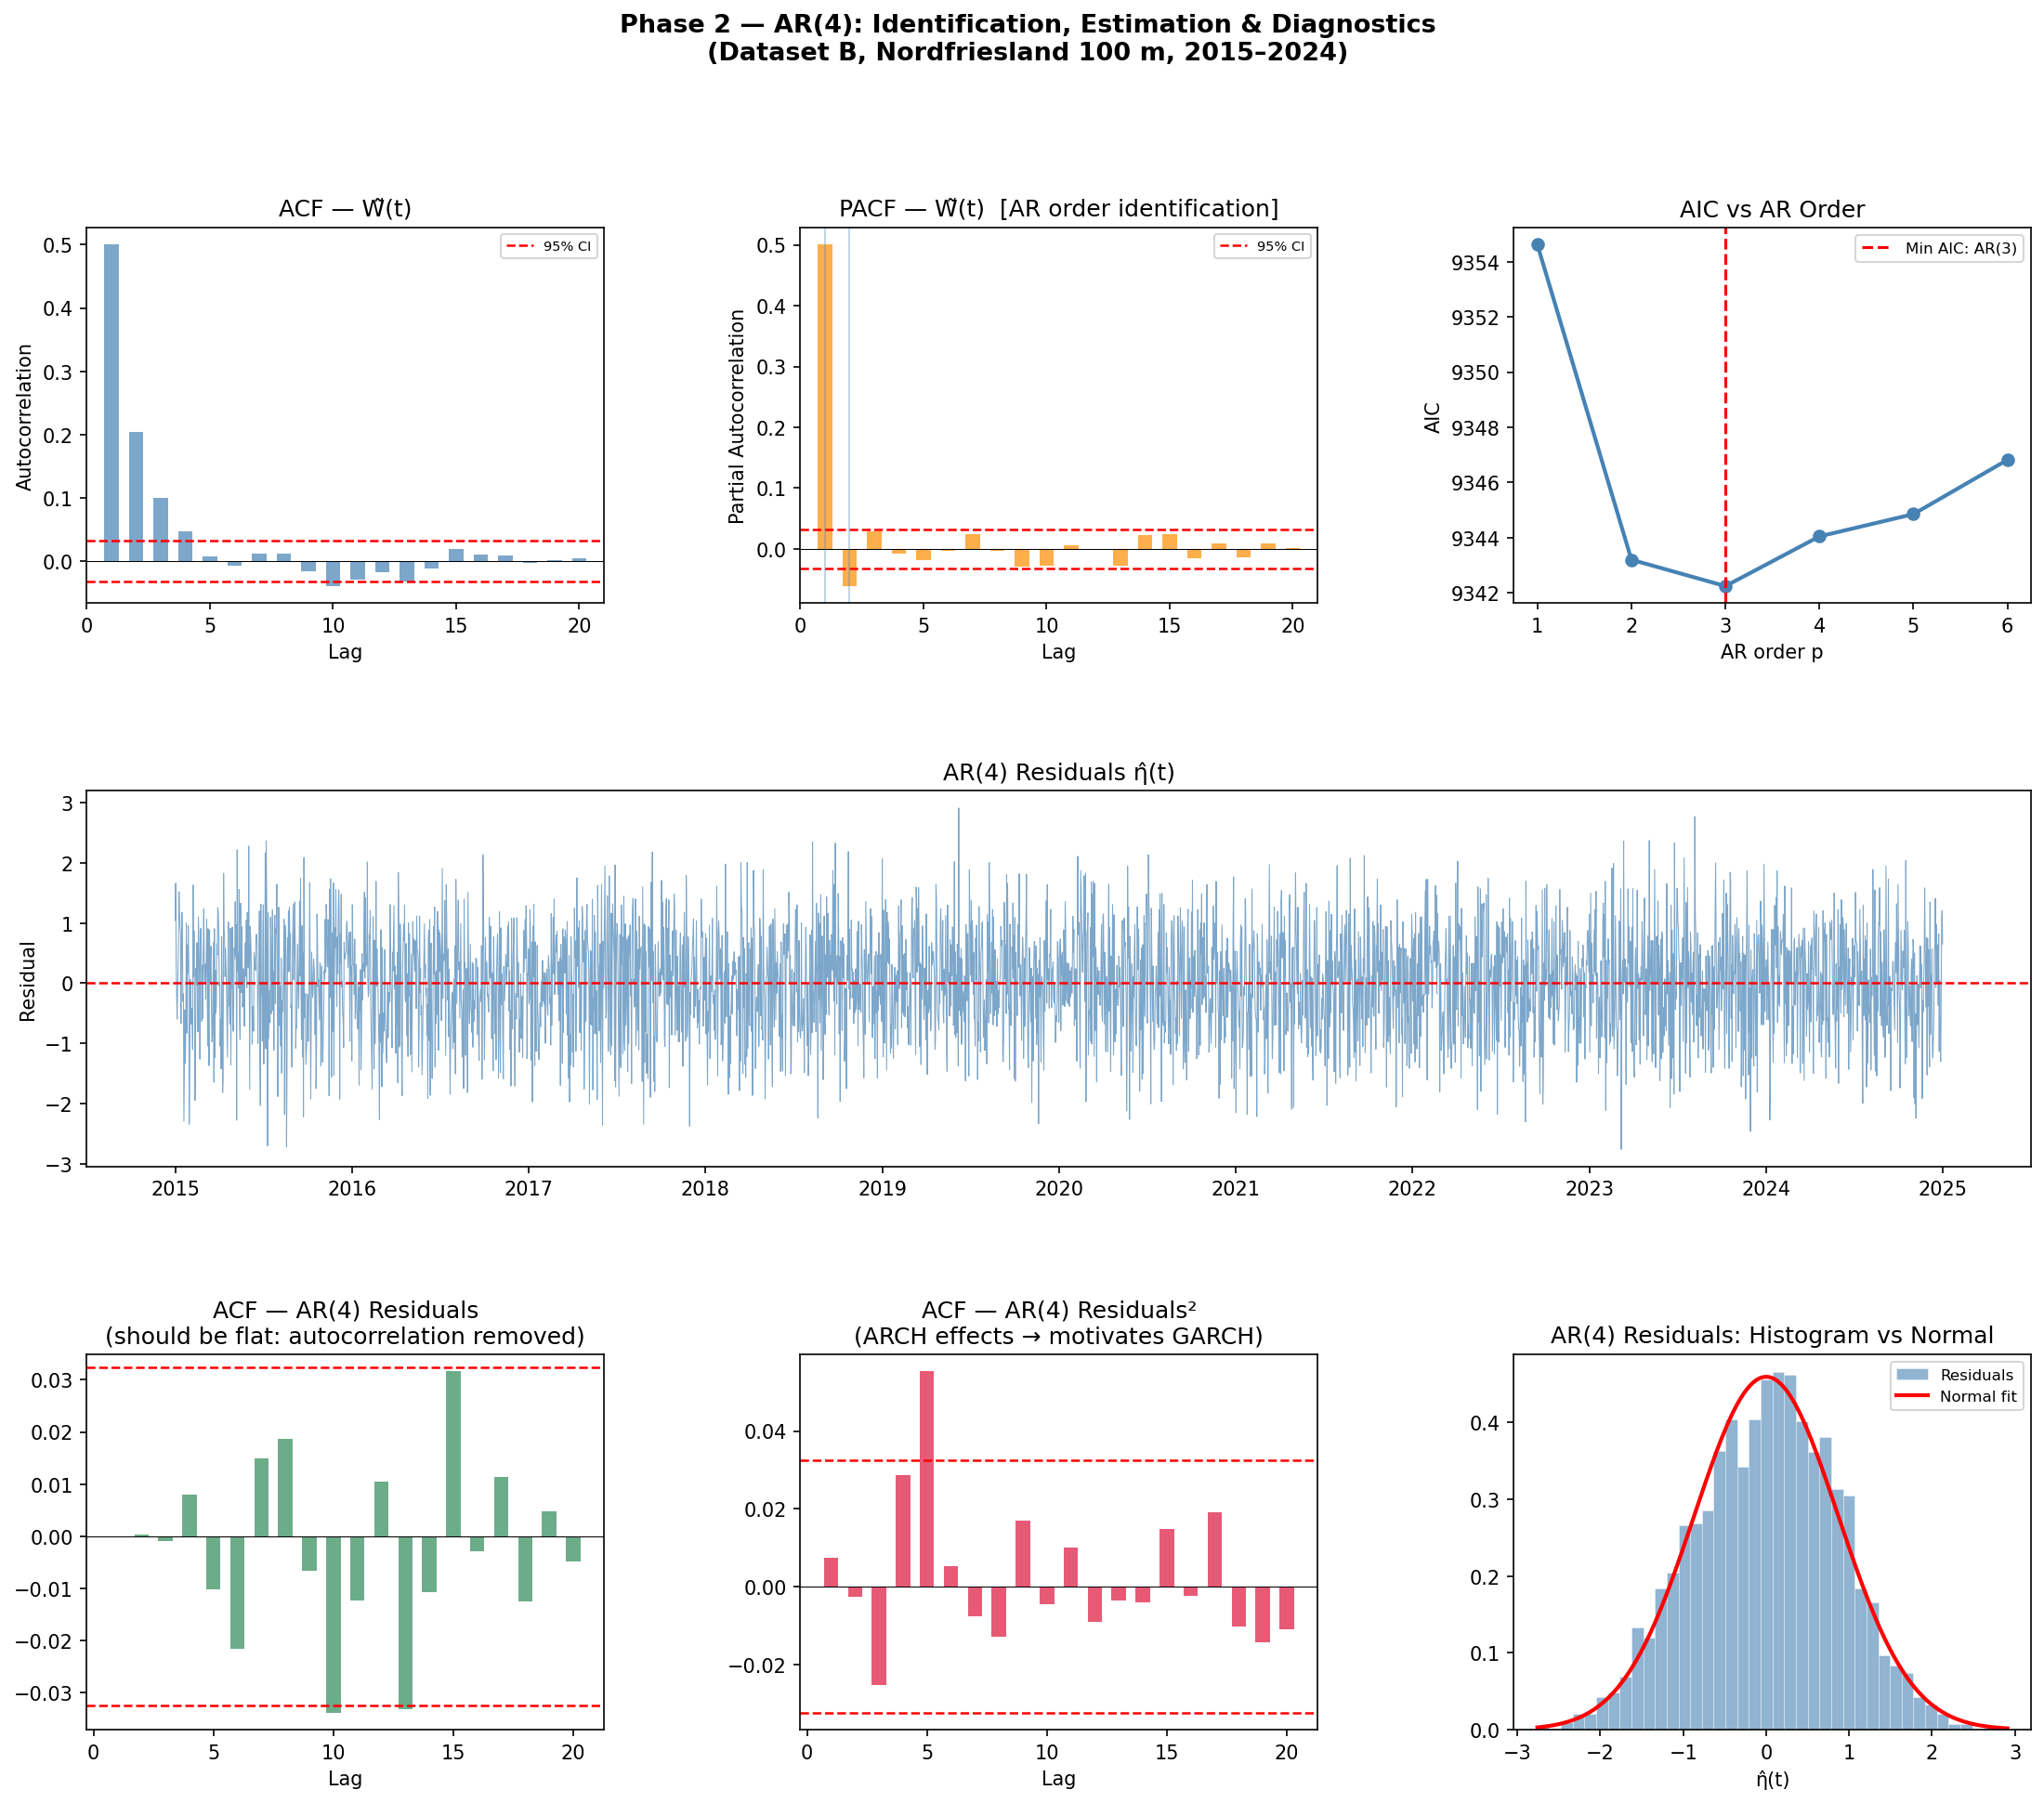
\includegraphics[width=0.9\textwidth]{../Plots/phase2_B_ar4_diagnostics.png}
\caption{AR(4) identification, estimation, and residual diagnostics. Top row: ACF and PACF showing sharp PACF cutoff at lag 4; AIC grid search confirming AR(4) optimality. Middle: time series of AR(4) residuals (white-noise-like). Bottom: ACF/PACF of residuals (flat, confirming autocorrelation removal) and ACF of squared residuals (prominent, indicating ARCH effects). Histogram of residuals with normal fit overlay.}
\label{fig:ar4_diag}
\end{figure}

\begin{figure}[h]
\centering
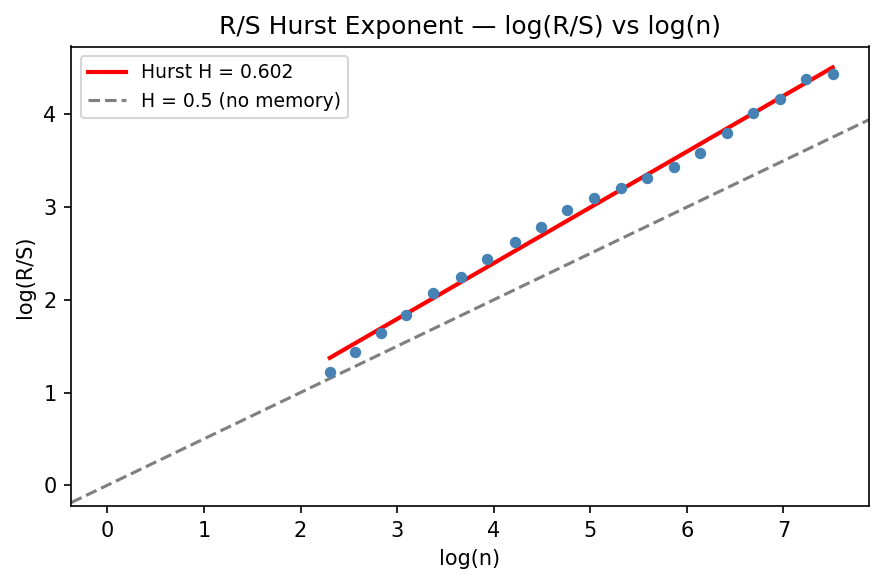
\includegraphics[width=0.9\textwidth]{../Plots/phase2_B_hurst_rs.png}
\caption{Rescaled-range (R/S) Hurst exponent analysis. Log-log scatter plot of $R/S$ vs window size, with fitted slope. H = 0.602 indicates persistence near the white-noise benchmark (H = 0.5), confirming absence of strong long-range dependence.}
\label{fig:hurst}
\end{figure}

\begin{figure}[h]
\centering
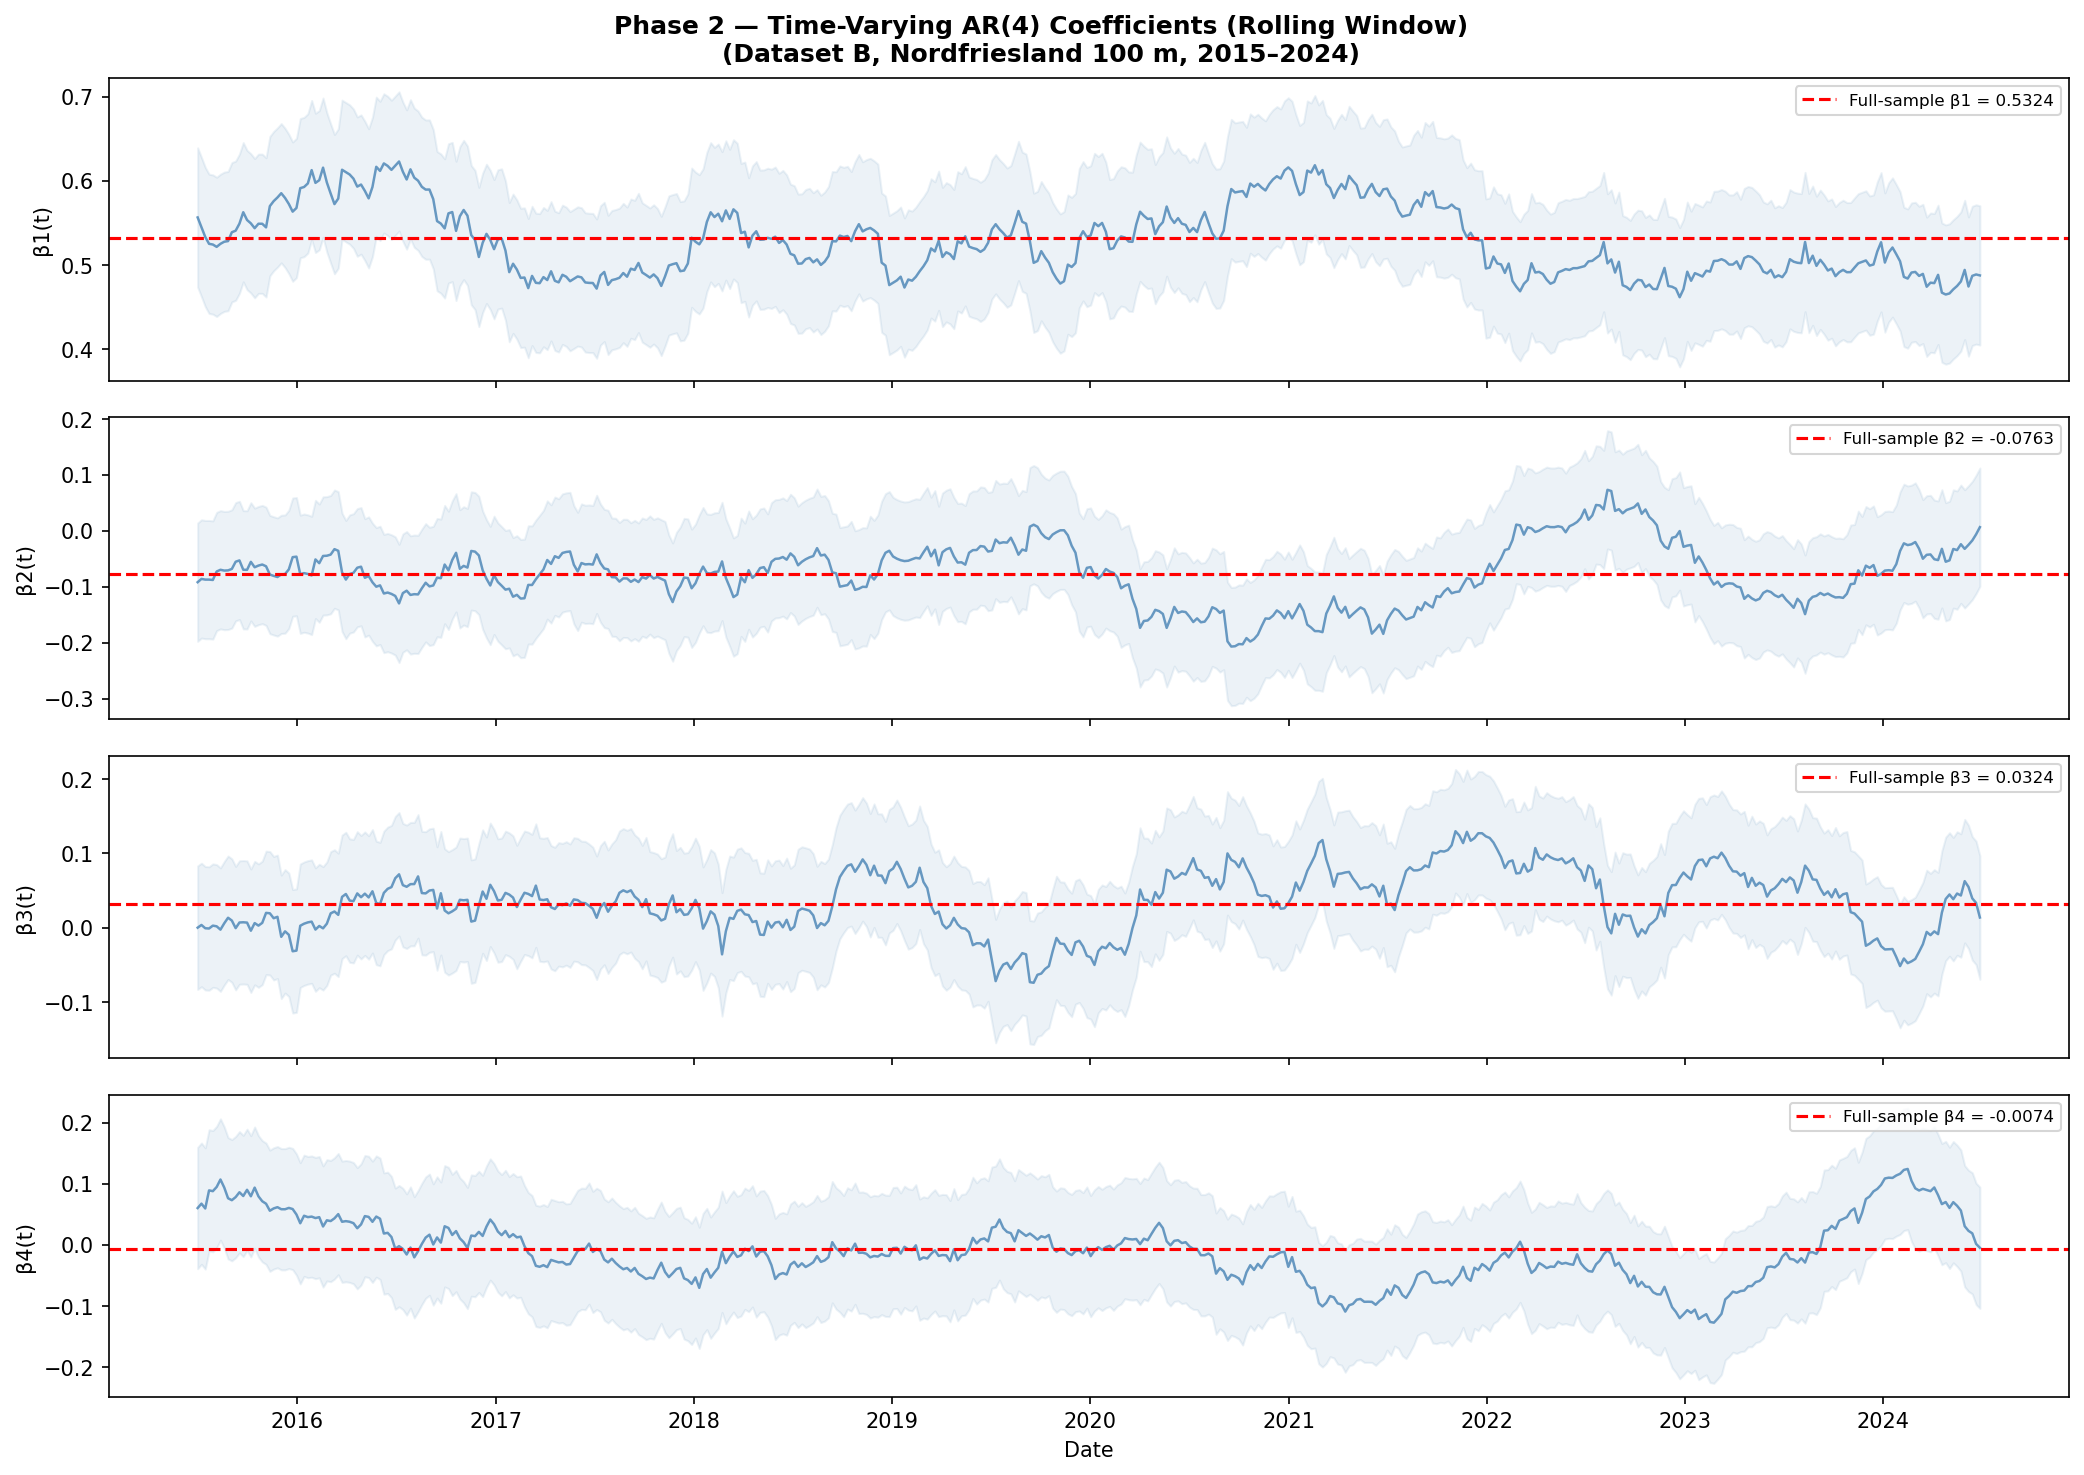
\includegraphics[width=0.9\textwidth]{../Plots/phase2_B_rolling_ar_coefficients.png}
\caption{Time-varying AR(4) coefficients over rolling 365-day windows. Each subplot shows $\beta_k(t)$ evolution, with red dashed line indicating the full-sample estimate. Bands around rolling coefficients represent two-standard-deviation confidence intervals. Seasonal variation in $\beta_1$ is visible; $\beta_2, \beta_3, \beta_4$ are relatively stable.}
\label{fig:rolling}
\end{figure}

\section{Conclusion}

Phase 2 successfully models the linear AR dynamics of standardised wind residuals. AR(4) is confirmed as the canonical model, with coefficients aligned to literature values and demonstrating superior out-of-sample forecasting performance (13.8\% RMSE gain over persistence, $p < 0.001$). Residual diagnostics confirm that (i) serial autocorrelation has been removed, (ii) conditional heteroskedasticity remains and requires GARCH treatment, and (iii) long memory is absent.

The AR(4) coefficients are fed directly into Phase 4 for CAR(4) continuous-time embedding via Euler discretisation. The detected ARCH effects will be explicitly modelled in Phase 3 (GARCH).

\section*{Data Availability}

Outputs from Phase 2 are saved to \texttt{reference\_nb/Phase\_2/}:
\begin{itemize}
  \item \texttt{ar4\_coefficients.csv}: $\beta_1, \beta_2, \beta_3, \beta_4$ with standard errors and $p$-values
  \item \texttt{ar4\_residuals\_phase2.csv}: Residuals $\widehat{\eta}(t)$ for Phase 3 (GARCH)
  \item \texttt{phase2\_B\_ar4\_diagnostics.png}: ACF/PACF, residual diagnostics
  \item \texttt{phase2\_B\_hurst\_rs.png}: R/S Hurst exponent
  \item \texttt{phase2\_B\_rolling\_ar\_coefficients.png}: Time-varying coefficient evolution
\end{itemize}

\newpage
\bibliographystyle{plainnat}
\begin{thebibliography}{99}

\bibitem[Alexandrinis (2013)]{Alexandrinis2013}
Alexandrinis, G. (2013).
\textit{Wind Derivatives: Modelling and Pricing}.
PhD Thesis, Technical University of Crete.

\bibitem[Benth \& Šaltytė Benth (2009)]{BenthSaltyteBenth2009}
Šaltytė~Benth, A., \& Benth, F.~E. (2009).
\textit{Stochastic Modelling of Temperature Variations with Applications to Weather Derivatives and Risk Management}.
Springer.

\bibitem[Diebold \& Mariano (1995)]{DM1995}
Diebold, F.~X., \& Mariano, R.~S. (1995).
Comparing predictive accuracy.
\textit{Journal of Business \& Economic Statistics}, 13(3), 253--263.

\bibitem[Engle (1982)]{Engle1982}
Engle, R.~F. (1982).
Autoregressive conditional heteroscedasticity with estimates of the variance of UK inflation.
\textit{Econometrica}, 50(4), 987--1007.

\bibitem[Torres et al. (2005)]{Torres2005}
Torres, J.~L., García, A., de Blas, M., \& de Francisco, A. (2005).
Forecast of hourly average wind speed with ARMA models in Navarre, Spain.
\textit{Solar Energy}, 79(1), 65--77.

\end{thebibliography}

\end{document}
